\documentclass[10pt,a4paper]{article}
\usepackage[utf8]{inputenc}
\usepackage[T1]{fontenc}
\usepackage[a4paper,top=1.5cm,bottom=1.5cm,left=1.5cm,right=1.5cm]{geometry}
\usepackage{amsmath}
\usepackage{amssymb}
\usepackage{tikz}
\usepackage{pgfplots}
\pgfplotsset{compat=1.18}
\pgfplotsset{
  grafik/.style={
    axis lines=middle,
    xlabel={$x$}, ylabel={$y$},
    width=7.5cm, height=6cm,
    grid=major, grid style={gray!25},
    tick label style={font=\scriptsize},
    every axis x label/.style={at={(ticklabel* cs:1)},anchor=west},
    every axis y label/.style={at={(ticklabel* cs:1)},anchor=south},
    title style={yshift=2ex},
  },
}
\usepackage[dvipsnames,svgnames]{xcolor}
\usepackage{booktabs}
\usepackage{tabularx}
\usepackage{array}
\usepackage[bookmarks=false]{hyperref}

\title{Rubrik Nilai Tugas Minggu 5 : Kekontinuan}
\author{Matematika untuk Sistem Informasi}
\date{}

\newenvironment{rubrik}{%
  \noindent
  \tabularx{\textwidth}{@{}>{\raggedright\arraybackslash}p{2.2cm}>{\raggedright\arraybackslash}X>{\centering\arraybackslash}p{1.1cm}>{\centering\arraybackslash}p{1.4cm}@{}}
  \toprule
  \textbf{Kriteria} & \textbf{Deskriptor} & \textbf{Maks} & \textbf{Skor} \\
  \midrule
}{%
  \bottomrule
  \endtabularx\par
}
\newcommand{\butir}[1]{\par\vspace{0.75em}\noindent\textbf{#1}\par\vspace{0.35em}}

\begin{document}
\maketitle

\noindent
Nama: \underline{\hspace{7.2cm}} \quad NIM: \underline{\hspace{4.2cm}}

\section*{Petunjuk penilai}
\begin{itemize}
  \item Tiap butir maksimum 100. Nilai tugas adalah rata-rata skor butir.
  \item Ketentuan skor:\par
  {\small
  \setlength{\tabcolsep}{4pt}%
  \begin{tabularx}{\linewidth}{@{}>{\raggedright\arraybackslash}p{2.1cm}>{\centering\arraybackslash}p{1.6cm}>{\raggedright\arraybackslash}X@{}}
  \toprule
  \textbf{Kriteria} & \textbf{Maks} & \textbf{Ketentuan} \\
  \midrule
  Langkah & 50 atau 60 & Jika langkah terbaca dan tidak seluruhnya salah, skor minimal 25. Skor di bawah 25 hanya bila langkah salah total, tidak dimengerti, atau tidak terbaca. \\
  Jawaban & 30 atau 40 & Harus ada dan benar. Skor hanya 0 atau nilai penuh. \\
  Penyajian & 20 & Harus ada dan benar. Skor hanya 0 atau nilai penuh. \\
  \bottomrule
  \end{tabularx}}
\end{itemize}

\[
f(x) =
\begin{cases}
  x^2 - 1, & x \leq -1 \\
  2x + 2, & x > -1
\end{cases}
\]
\butir{Butir 1. Kekontinuan $f$ di $x = -1$ (100 poin)}
\begin{rubrik}
Langkah &
Tiga syarat: $f(-1)$ terdefinisi, limit kiri sama dengan limit kanan, dan limit sama dengan nilai fungsi. &
60 & \\
Jawaban &
$f(-1) = 0$, kedua limit sama dengan $0$, sehingga $f$ kontinu di $x = -1$. &
40 & \\
\midrule
\multicolumn{2}{r}{\textbf{Jumlah}} & 100 & \\
\end{rubrik}

\[
f(x) =
\begin{cases}
  2x, & x \leq -1 \\
  x^2 - 1, & -1 < x < 2 \\
  4 - x, & x \geq 2
\end{cases}
\]
\butir{Butir 2(a). Grafik fungsi (100 poin)}
\begin{rubrik}
Langkah &
Ujung tiap potongan dihitung: penuh $(-1,-2)$ dan $(2,2)$, kosong $(-1,0)$ dan $(2,3)$. &
50 & \\
Jawaban &
Grafik melompat di $x = -1$ dan di $x = 2$. &
30 & \\
Penyajian &
Gambar memuat garis, parabola, dan garis dengan titik penuh serta titik kosong yang sesuai.\par\vspace{0.4em}
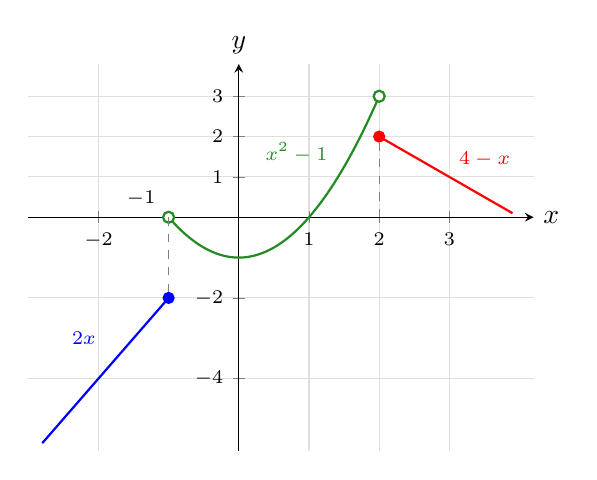
\begin{tikzpicture}
\begin{axis}[grafik, width=8cm, height=6.5cm, xmin=-3, xmax=4.2, ymin=-5.8, ymax=3.8,
  xtick={-2,1,2,3}, ytick={-4,-2,1,2,3}]
  \addplot[domain=-2.8:-1, thick, blue] {2*x};
  \addplot[domain=-1:2, samples=80, thick, ForestGreen] {x^2 - 1};
  \addplot[domain=2:3.9, thick, Red] {4 - x};
  \filldraw[blue] (axis cs:-1,-2) circle (2pt);
  \filldraw[ForestGreen, fill=white, thick] (axis cs:-1,0) circle (2pt);
  \filldraw[ForestGreen, fill=white, thick] (axis cs:2,3) circle (2pt);
  \filldraw[Red] (axis cs:2,2) circle (2pt);
  \draw[dashed, gray] (axis cs:-1,0) -- (axis cs:-1,-2);
  \node[font=\scriptsize, anchor=south east] at (axis cs:-1.05,0.05) {$-1$};
  \draw[dashed, gray] (axis cs:2,0) -- (axis cs:2,2);
  \node[font=\scriptsize, blue, anchor=east] at (axis cs:-1.9,-3) {$2x$};
  \node[font=\scriptsize, ForestGreen, anchor=east] at (axis cs:1.4,1.6) {$x^2 - 1$};
  \node[font=\scriptsize, Red, anchor=south west] at (axis cs:3,1) {$4 - x$};
\end{axis}
\end{tikzpicture} &
20 & \\
\midrule
\multicolumn{2}{r}{\textbf{Jumlah}} & 100 & \\
\end{rubrik}

\butir{Butir 2(b). Kekontinuan di $x = -1$ dan $x = 2$ (100 poin)}
\begin{rubrik}
Langkah &
Di tiap titik, nilai fungsi serta limit kiri dan kanan dibandingkan. &
60 & \\
Jawaban &
Tidak kontinu di $x = -1$ (kontinu kiri); tidak kontinu di $x = 2$ (kontinu kanan). Keduanya diskontinuitas lompat. &
40 & \\
\midrule
\multicolumn{2}{r}{\textbf{Jumlah}} & 100 & \\
\end{rubrik}

\butir{Butir 3. Konstanta $a$ dan $b$ agar $f$ kontinu di $\mathbb{R}$ (100 poin)}
\[
f(x) =
\begin{cases}
  \dfrac{x^2 - 4}{x - 2}, & x < 2 \\[1.5ex]
  ax^2 - bx + 3, & 2 \leq x < 3 \\
  2x - a + b, & x \geq 3
\end{cases}
\]
\begin{rubrik}
Langkah &
Pecahan disederhanakan untuk $x \neq 2$, syarat kontinu ditulis di $x = 2$ dan $x = 3$, lalu sistem diselesaikan. &
60 & \\
Jawaban &
$a = \frac{1}{2}$ dan $b = \frac{1}{2}$. &
40 & \\
\midrule
\multicolumn{2}{r}{\textbf{Jumlah}} & 100 & \\
\end{rubrik}

\[
f(x) =
\begin{cases}
  x + 3, & x \leq -1 \\
  -x + c, & -1 < x < 1 \\
  x^2 - 2x + 1, & x \geq 1
\end{cases}
\]
\butir{Butir 4(a). Nilai $c$ agar kontinu di $x = -1$ (100 poin)}
\begin{rubrik}
Langkah &
$f(-1)$ dan limit kanan $-x + c$ disamakan. &
60 & \\
Jawaban &
$c = 1$. &
40 & \\
\midrule
\multicolumn{2}{r}{\textbf{Jumlah}} & 100 & \\
\end{rubrik}

\butir{Butir 4(b). Kekontinuan di $x = 1$ untuk $c$ pada (a) (100 poin)}
\begin{rubrik}
Langkah &
Dengan $c = 1$, nilai $f(1)$ serta limit kiri dan kanan dibandingkan. &
60 & \\
Jawaban &
Ketiga syarat terpenuhi, sehingga $f$ kontinu di $x = 1$. &
40 & \\
\midrule
\multicolumn{2}{r}{\textbf{Jumlah}} & 100 & \\
\end{rubrik}

\butir{Butir 5. Empat grafik: kontinu kiri, kontinu kanan, atau tidak kontinu (100 poin)}
\begin{center}
\begin{tabular}{cc}
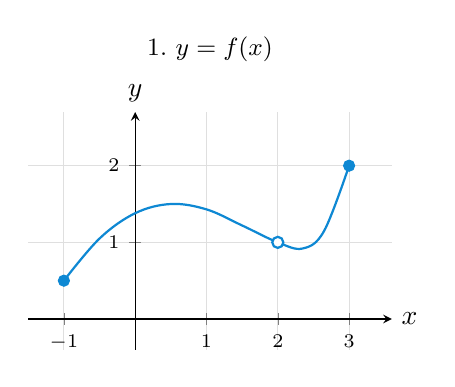
\begin{tikzpicture}
\begin{axis}[grafik, width=6.2cm, height=4.6cm, clip=false, xmin=-1.5, xmax=3.6, ymin=-0.4, ymax=2.7,
  xtick={-1,...,3}, ytick={1,2}, title={\small 1.\ $y = f(x)$}]
  \addplot[thick, cyan!70!blue, smooth, tension=0.6] coordinates
    {(-1,0.5) (-0.5,1.05) (0,1.38) (0.5,1.5) (1,1.43) (1.5,1.22) (2,1) (2.35,0.92) (2.65,1.15) (3,2)};
  \filldraw[cyan!70!blue] (axis cs:-1,0.5) circle (2pt);
  \filldraw[cyan!70!blue, fill=white, thick] (axis cs:2,1) circle (2pt);
  \filldraw[cyan!70!blue] (axis cs:3,2) circle (2pt);
\end{axis}
\end{tikzpicture}
&
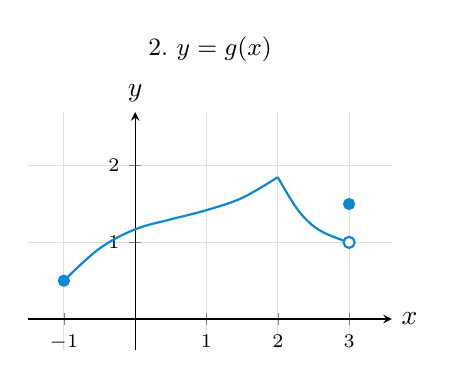
\begin{tikzpicture}
\begin{axis}[grafik, width=6.2cm, height=4.6cm, clip=false, xmin=-1.5, xmax=3.6, ymin=-0.4, ymax=2.7,
  xtick={-1,...,3}, ytick={1,2}, title={\small 2.\ $y = g(x)$}]
  \addplot[thick, cyan!70!blue, smooth, tension=0.6] coordinates
    {(-1,0.5) (-0.5,0.92) (0,1.17) (0.5,1.3) (1,1.42) (1.5,1.58) (2,1.85)};
  \addplot[thick, cyan!70!blue, smooth, tension=0.6] coordinates
    {(2,1.85) (2.3,1.4) (2.6,1.15) (3,1)};
  \filldraw[cyan!70!blue] (axis cs:-1,0.5) circle (2pt);
  \filldraw[cyan!70!blue, fill=white, thick] (axis cs:3,1) circle (2pt);
  \filldraw[cyan!70!blue] (axis cs:3,1.5) circle (2pt);
\end{axis}
\end{tikzpicture}
\\[2ex]
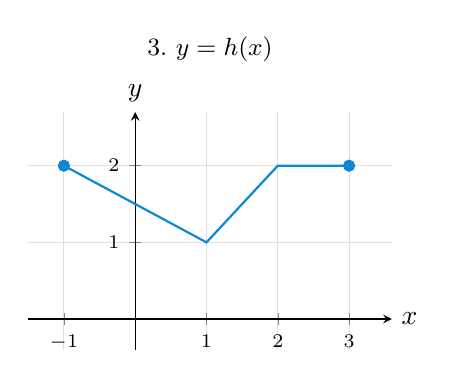
\begin{tikzpicture}
\begin{axis}[grafik, width=6.2cm, height=4.6cm, clip=false, xmin=-1.5, xmax=3.6, ymin=-0.4, ymax=2.7,
  xtick={-1,...,3}, ytick={1,2}, title={\small 3.\ $y = h(x)$}]
  \addplot[thick, cyan!70!blue, no marks] coordinates {(-1,2) (1,1) (2,2) (3,2)};
  \filldraw[cyan!70!blue] (axis cs:-1,2) circle (2pt);
  \filldraw[cyan!70!blue] (axis cs:3,2) circle (2pt);
\end{axis}
\end{tikzpicture}
&
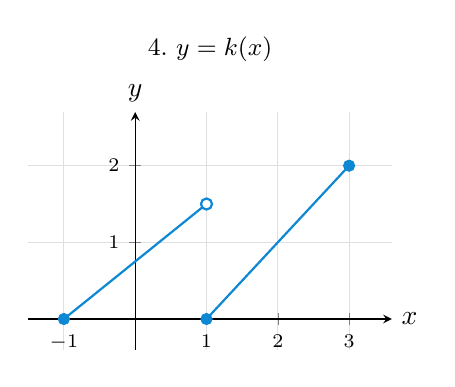
\begin{tikzpicture}
\begin{axis}[grafik, width=6.2cm, height=4.6cm, clip=false, xmin=-1.5, xmax=3.6, ymin=-0.4, ymax=2.7,
  xtick={-1,...,3}, ytick={1,2}, title={\small 4.\ $y = k(x)$}]
  \addplot[thick, cyan!70!blue, no marks] coordinates {(-1,0) (1,1.5)};
  \addplot[thick, cyan!70!blue, no marks] coordinates {(1,0) (3,2)};
  \filldraw[cyan!70!blue] (axis cs:-1,0) circle (2pt);
  \filldraw[cyan!70!blue, fill=white, thick] (axis cs:1,1.5) circle (2pt);
  \filldraw[cyan!70!blue] (axis cs:1,0) circle (2pt);
  \filldraw[cyan!70!blue] (axis cs:3,2) circle (2pt);
\end{axis}
\end{tikzpicture}
\end{tabular}
\end{center}
\begin{rubrik}
Langkah &
Di tiap titik sambung atau ujung, nilai fungsi dibedakan dari arah kurva yang menuju titik itu. &
60 & \\
Jawaban &
$f$: kontinu kanan di $-1$, tidak kontinu di $2$, kontinu kiri di $3$.
$g$: kontinu kanan di $-1$, kontinu di $2$, tidak kontinu di $3$.
$h$: kontinu pada $[-1, 3]$.
$k$: kontinu kanan di $-1$, tidak kontinu di $1$ (lompat), kontinu kiri di $3$. &
40 & \\
\midrule
\multicolumn{2}{r}{\textbf{Jumlah}} & 100 & \\
\end{rubrik}

\section*{Rekap skor}
\noindent
\begin{tabular}{@{}lr@{}}
\toprule
Butir & Skor \\
\midrule
1 & \\
2(a) & \\
2(b) & \\
3 & \\
4(a) & \\
4(b) & \\
5 & \\
\midrule
Rata-rata = jumlah skor / 7 (maksimum 100) & \\
\bottomrule
\end{tabular}

\end{document}
